% !TEX root = ../thesis-example.tex
%
\chapter{Theorie/Begriffsbestimmung}
\label{sec:theorie:Theorie}

\cleanchapterquote{Most good programmers do programming not because they expect to get paid or get adulation by the public, but because it is fun to program.}{Linus Torvalds}{(Finnish American, software engineer and hacker)}

Um das allgemeine Verständnis zu gewährleisten müssen noch einige wichtige Begriffe geklärt werden, die die Grundlage für die folgende Untersuchung bilden.

Die Entscheidung, welche der mobilen Variante man für die Umsetzung verwendet ist abhängig von den jeweiligen Eigenschaften. Auf wieviel Speicher darf die App zugreifen, welche Handyfunktionen werden benötigt und lässt sich feststellen wann eine Internetverbindung besteht und lassen sich davon abhängig die Daten mit dem Server abgleichen.

\section{Native Apps}
\label{sec:intro:native}

Die Nativen Apps werden speziell für das jeweilige Betriebssystem entwickelt z.B. iOS oder Android. Diese laufen dann auch ausschließlich auf iOS Geräten wie dem iPhone und dem iPad, oder Android Geräten wie dem Samsung Galaxy S4.\cite[]{WEB:APPEV:2014}

Dadurch stellt man eine optimale Nutzung der Ressourcen und einheitlich funktionierende Hardwareschnittstellen sicher.\cite[]{WEB:APPEV:2014}

\subsection{Vorteile}
\label{sec:native:pros}

\begin{itemize}

	\item Native Apps nutzen die Leistung des Betriebssystems und des verwendeten Gerätes voll aus, da sie speziell für das Betriebssystem angepasst sind. Dadurch lassen sich sehr gut komplexere und rechenintensivere Apps umsetzen.\cite[]{WEB:APPEV:2014}

	\item Durch die Installation der Apps auf dem Endgerät, können Hardwarefunktionen wie Kamera, Beschleunigungssensor oder \ac{GPS} benutzt werden. Das ist in der Regel nur nativen Apps vorbehalten.\cite[]{WEB:APPEV:2014}

	\item Daten können auf dem Endgerät in beliebiger Menge gespeichert werden.\cite[]{WEB:APPEV:2014}

	\item Da Native Apps über einen Appstore vertrieben werden, werden diese öfter gekauft, wenn Sie über gute Bewertungen verfügen.\cite[]{WEB:APPEV:2014}

	\item Die App lässt sich sehr einfach über den Appstore installieren und es wird automatisch ein Icon zum Starten angelegt.\cite[]{WEB:APPEV:2014}

	\item Der Vertriebsaufwand ist sehr gering, da die Appstores verbreitete Bezugsquellen für Native Apps sind. Ist die App erfolgreich, kann man sich in den Top-Listen der App Stores wiederfinden und dadurch sehr hohe Downloadzahlen erreichen.\cite[]{WEB:APPEV:2014}

\end{itemize}

\subsection{Nachteile}
\label{sec:native:cons}

\begin{itemize}

	\item Ein großer Nachteil ist der erforderliche Entwicklungsaufwand, wenn man die App in allen Appstores anbieten möchte. Dafür muss man die App an die jeweiligen Gegebenheiten des Betriebssystems optimieren.\cite[]{WEB:APPEV:2014}

	\item Es entstehen zusätzliche Kosten um die App für den entsprechenden entwicklen und anbieten zu können.

\end{itemize}

\section{Webapps}
\label{sec:intro:webapp}

Die sogenannten Webapps sind im eigentlichen Sinne speziell programmierte \ac{HTML5} Websites, die erkennen auf welchem Endgerät sie aufgerufen werden und optimieren den Inhalt entsprechend. Somit kann quasi jedes mobile Endgerät, dass über einen Webbrowser verfügt, die App nutzen.

\subsection{Vorteile}
\label{sec:webapp:pros}

\begin{itemize}

	\item Web Apps sind quasi unabhängig vom Betriebssystem und funktionieren auf allen Smartphones. Dadurch erreicht man mehr potentielle Nutzer, bei gleichzeitig geringeren Kosten.\cite[]{WEB:APPEV:2014}

	\item In der Regel kommt man mit der Entwicklung einer Web App günstiger, als mit der Entwicklung einer nativen App für nur ein Betriebssystem.\cite[]{WEB:APPEV:2014}

	\item Durch die Verwendung von HTML5 wird auch die Offline-Speicherung von Daten ermöglicht. Somit kann man auch ohne permanente Internetverbindung die einmal geladene Web App nutzen.\cite[]{WEB:APPEV:2014}

	\item Über Onlinesuchmaschinen wie z.B. Google können Web Apps ohne großen Aufwand gefunden werden und lassen sich auch ohne Installation direkt nutzen. Speichert man diese als Lesezeichen, lässt sie sich genau wie eine Native App vom Startbildschirm aus starten.\cite[]{WEB:APPEV:2014}

	\item Die Veröffentlich und Aktualisierung erfolgt in Sekundenschnelle, da sie im Gegensatz zu Nativen Apps keinen Zulassungsprozess durchlaufen müssen.\cite[]{WEB:APPEV:2014}

	\item Vertreibt man die App selbst, entfällt die Provision von überlicherweise 30\% an den Betreiber des App Stores.\cite[]{WEB:APPEV:2014}

	\item Hat man vor die irgendwann die Vorteile einer nativen App zu nutzen und beachtet das bei der Programmierung der Web App, lässt sich diese leicht und kostengünstig in eine Native App umwandeln.\cite[]{WEB:APPEV:2014}

\end{itemize}

\subsection{Nachteile}
\label{sec:webapp:cons}

\begin{itemize}

	\item Die meisten Hardwarefunktionen der mobilen Geräte lassen sich garnicht oder nur mit spezieller Zustimmung des Nutzers verwenden.\cite[]{WEB:APPEV:2014}

	\item Komplexe Berechnungen wie z.B. 3D Darstellungen, Verschlüsselung oder Bildbearbeitungen sind mit einer Web App nicht möglich.\cite[]{WEB:APPEV:2014}

	\item Benötigt die App mehr als 10MB an Datenmaterial auf dem Endgerät ist von einer Entwicklung als reine Web App abzusehen.\cite[]{WEB:APPEV:2014}

	\item Geschäftsmodelle die auf In-App-Käufe oder einen App Store aufbauen, funktionieren zusammen mit der Web App nicht.\cite[]{WEB:APPEV:2014}

\end{itemize}

\section{Hybridapps}
\label{sec:intro:hybrid}

Hybridapps sollen die Vorteile der Web App Entwicklung und der Entwicklung von nativen Apps in sich vereinen. Dabei setzen die Entwickler auf eine große Anzahl von Frameworks. PhoneGap, Corona oder Appelerator Titanium sind Beispiele dafür, mit deren Hilfe man Web Apps in eine native App umwandeln kann.

Für Einige mag die Entwicklung einer Hybridapp als \"Allheilmittel\" klingen, jedoch gibt es auch hier Vor- und Nachteile.\cite[]{WEB:APPEV:2014}

\subsection{Vorteile}
\label{sec:hybrid:pros}

\begin{itemize}

	\item Durch die Verwendung einer Hybrid App lässt sich eine Cross Browser Web App erstellen, die in allen modernen Browsern läuft.\cite[]{WEB:APPEV:2014}

	\item Da eine Web App mittels Frameworks für verschiedene Betriebssysteme umgewandelt werden kann, erspart man sich die eigenständige Entwicklung für jedes einzelne Betriebssystem. Es bleiben im schlimmsten Fall nur Betriebssystemspezifische Feinheiten, die noch angepasst werden müssen.\cite[]{WEB:APPEV:2014}

	\item Mit Javascript lassen sich viele Hardwarefunktionen der Endgeräte nutzen, auf die man bei einer Web App nicht zugreifen konnte.\cite[]{WEB:APPEV:2014}

	\item Der Verkauf einer Hybrid App kann wieder über den jeweiligen App Store erfolgen.\cite[]{WEB:APPEV:2014}

\end{itemize}

\subsection{Nachteile}
\label{sec:hybrid:cons}

\begin{itemize}

	\item Ein großer Nachteil der Hybridapps kann entstehen, wenn man sehr rechenintensive Anwendungen verwendet. Dadurch können Hybrid Apps sehr schnell an das Leistungsmaximum herranreichen und träge reagieren. Das ist sehr stark von dem verwendeten Framwork abhängig und ein Nachteil der in Zukunft durch merklich effizienter werdende Frameworks behoben werden kann.\cite[]{WEB:APPEV:2014}

	\item Die Progammierung einer Hybrid App könnte mit zunehmendem Komplexitätsgrad sehr aufwendig werden und eine Umsetzung mittels nativer App empfehlenswerter machen.\cite[]{WEB:APPEV:2014}

\end{itemize}

\section{Wahl der Appvariante}
\label{sec:intro:Appvariante}

Die Wahl der Appvariante ist nicht allein abhängig von den Vor- und Nachteilen der Varianten. Hierfür muss man auch die bestehende Website betrachten und die Umsetzungsaufwände gegeneinander abwägen.

Ein nicht zu unterschätzender Vorteil der Website ist die bereits responsive Umsetzung. Dadurch passt sich der dargestellte Inhalt an das Endgerät an, wodurch optimale Darstellung auch auf mobilen Geräten gewährleistet wird. Es können somit bereits neue Daten mobil erfasst werden.

\begin{figure}[htb]
	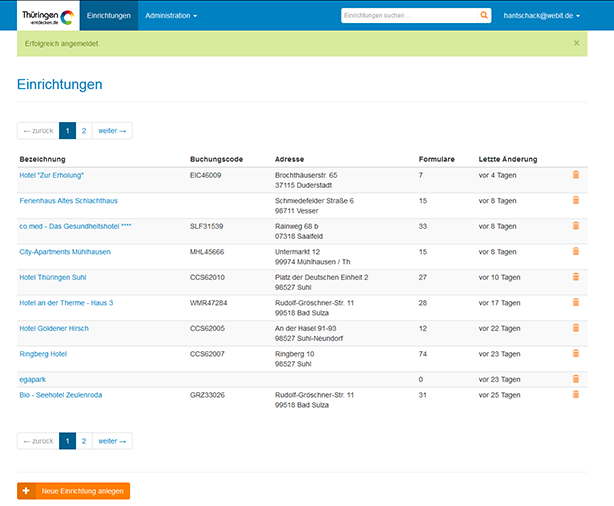
\includegraphics[width=\textwidth]{Bilder/Barrierefreidatenbank}
	\caption{Barrierefreiheitsdatenbank}
	\label{fig:system:Barrierefreidatenbank}
\end{figure}

\begin{figure}[htb]
	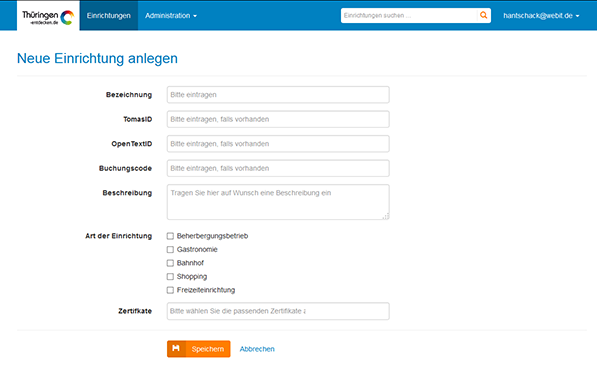
\includegraphics[width=\textwidth]{Bilder/Datenerfassung}
	\caption{Datenerfassung}
	\label{fig:system:Datenerfassung}
\end{figure}

\begin{figure}[htb]
	\begin{tabular}{l r}
		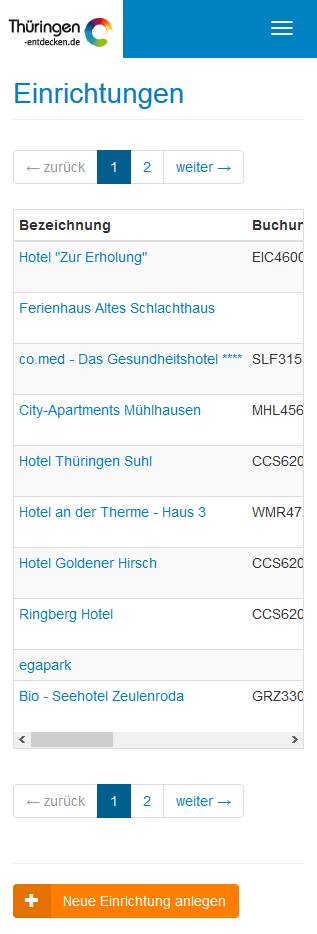
\includegraphics[width=0.49\textwidth]{Bilder/Barrierefreidatenbank-mobil}
		&
		
\includegraphics[width=0.49\textwidth]{Bilder/Datenerfassung-mobil}
	\end{tabular}
	\caption{Barrierefreiheitsdatenbank mobil}
\end{figure}

Nach Betrachtung der Vor- und Nachteile der App Varianten und der bestehenden Website, schließe ich die Umsetzung einer reinen nativen App aus. Der Umsetzungsaufwand und die entstehenden Kosten wären unangemessen hoch im Vergleich zu den daraus entstehenden Vorteilen.